\section{Bifurcations}
\label{sec:arch.bif}

This section explores the bifurcations that happen at the borders of ``type A'' and ``type B'' parameter regions, respectively.
\Cref{fig:arch.dyn.regions.full} shows the borders of the parameter regions in full.
\Cref{fig:arch.dyn.regions.zoomed} is a zoomed-in version, that pictures the parameter region that contain the point $F_{16}$ of \Cref{fig:arch.dyn.period}.
It is a ``type B'' parameter region with the stable cycles $\Cycle{\A^5\B^3\C^4\D^4}$ and $\Cycle{\A^4\B^4\C^5\D^3}$.
Every one of its boundaries has a ``type A'' parameter region on the other side.
Therefore, we only need to describe the 4 boundaries of this ``type B'' parameter region in depth to cover all the boundaries of both ``type A'' and ``type B'' parameter regions.

\begin{figure}
	\centering
	\subfloat[Full]{
		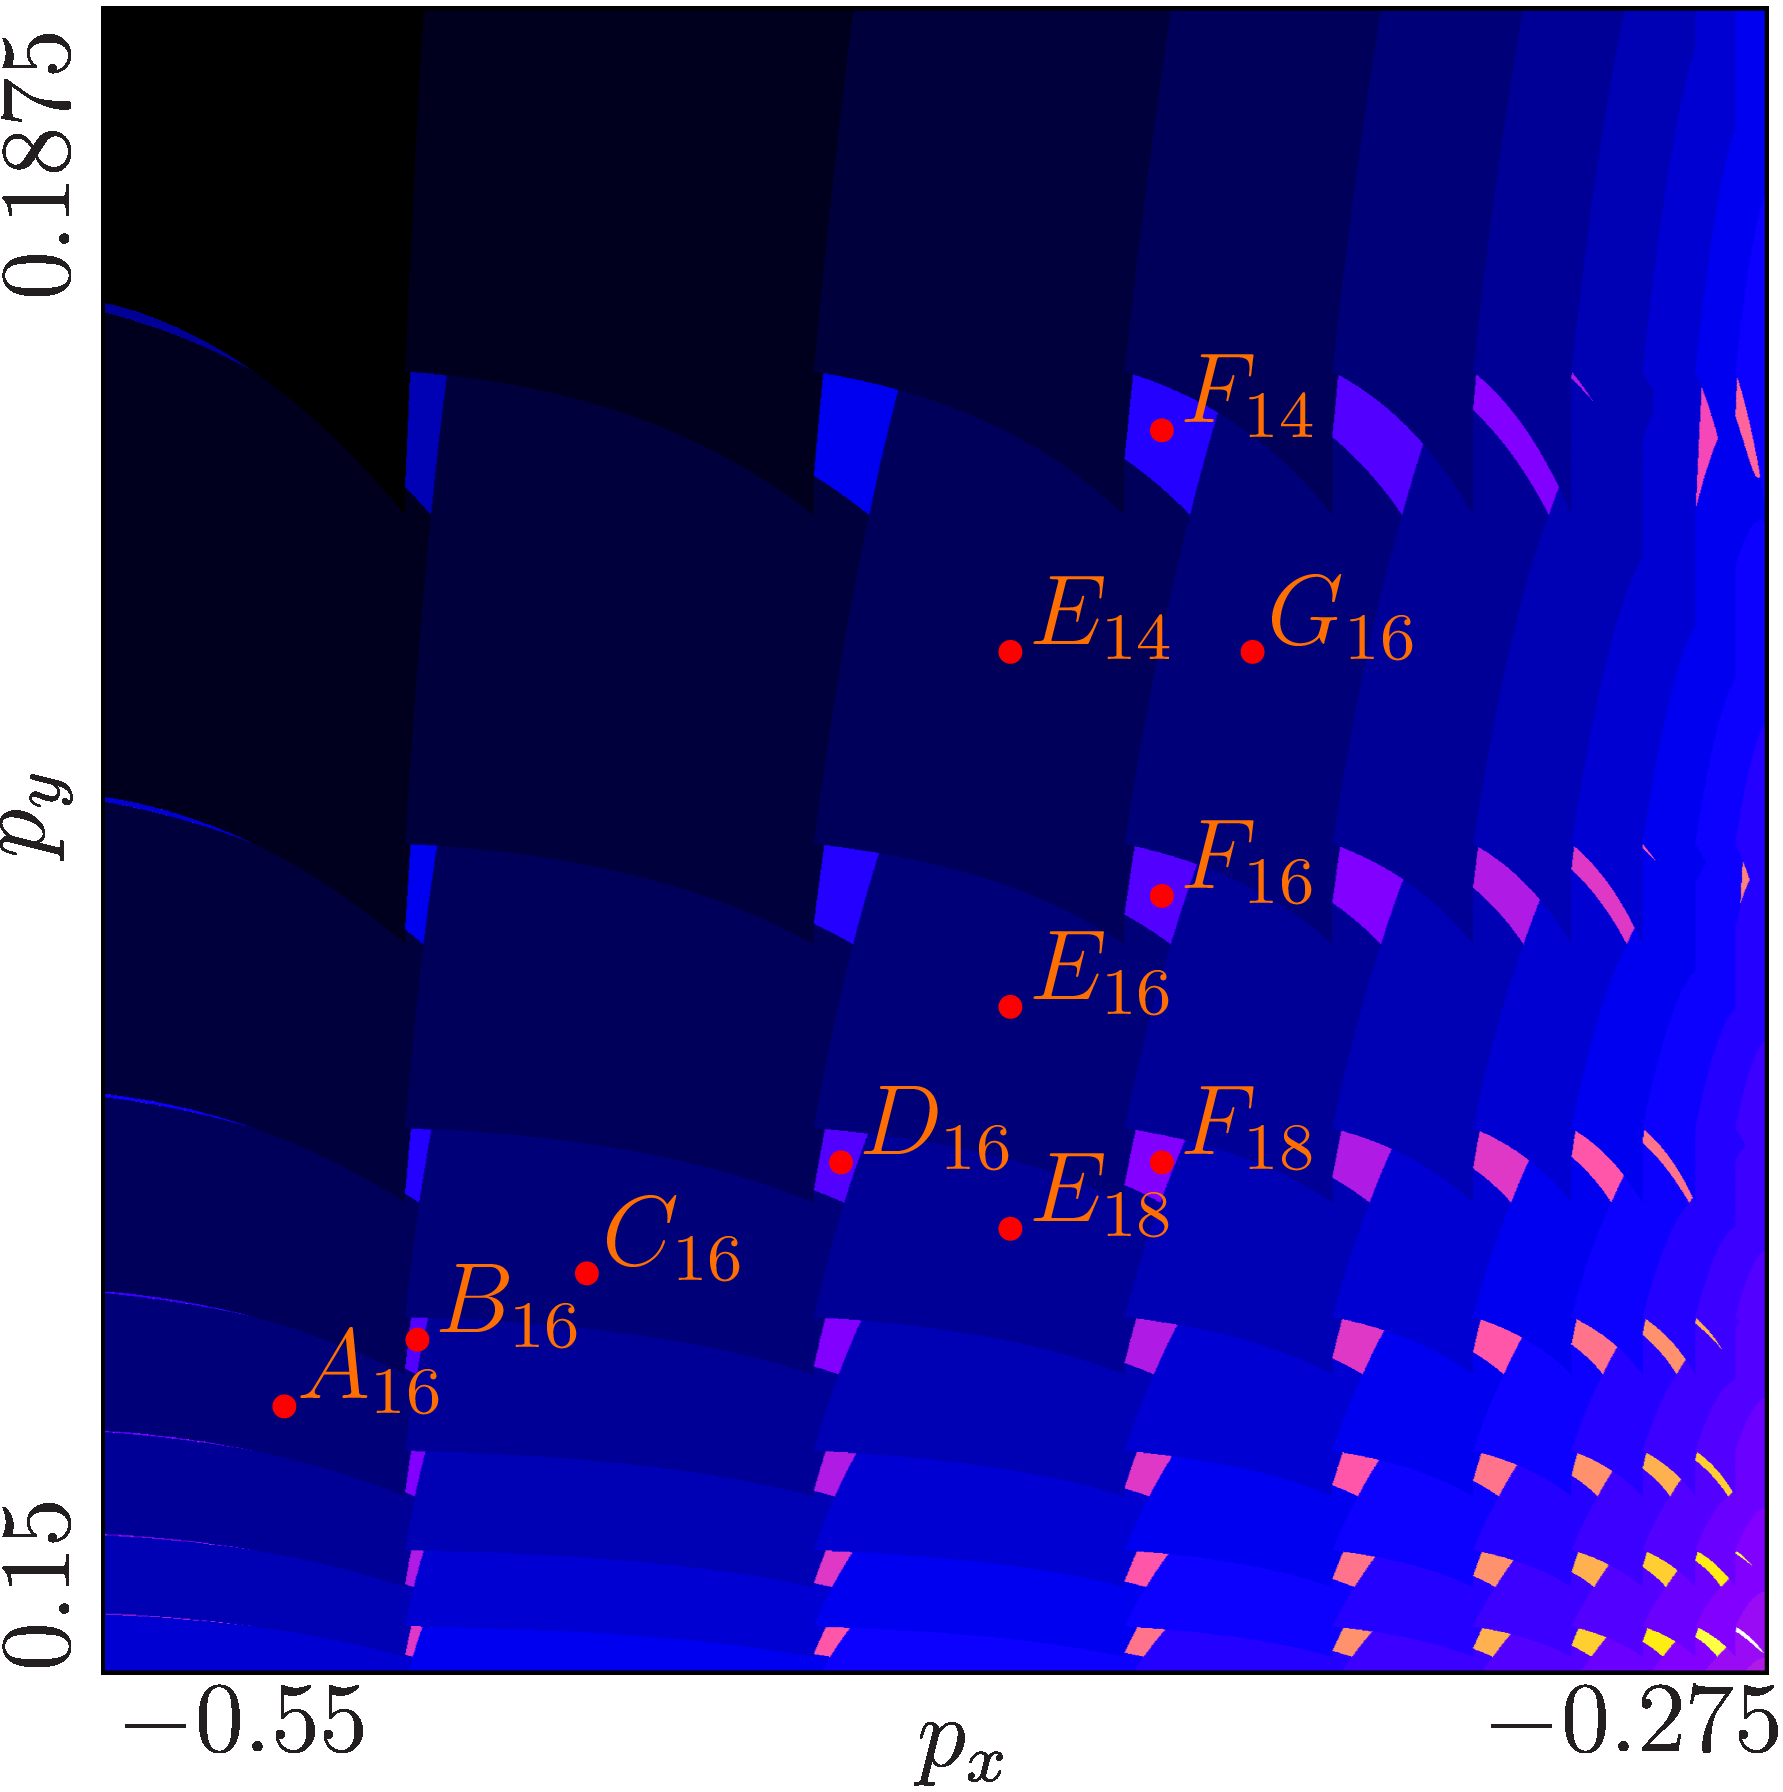
\includegraphics[width=.4\textwidth]{60_MinimalRepr/2D_Regions_Whole/result-halved.png}
		\label{fig:arch.dyn.regions.full}
	}
	\subfloat[Zoomed-in]{
		\includegraphics[width=.4\textwidth]{60_MinimalRepr/2D_Regions_F_Boundaries/result.png}
		\label{fig:arch.dyn.regions.zoomed}
	}
	\caption[2D scans of the boundaries of parameter regions with different symbolic sequences in the archetypal model]{
		2D scans of the boundaries of parameter regions with different symbolic sequences in the archetypal model.
		The parameters $a_L = 4, b_L = -\frac{1}{2},$ and $g_R\left(\frac{1}{4}\right) = 0.525$ are fixed.
		In (a), the parameters $\alpha = -g_R\left(\frac{1}{4}\right)$ and $\beta = c_L$ are varied in the ranges $[-0.55, -0.275]$ and $[0.15, 0.1875]$, respectively.
		(b) is a zoomed-in version with the same parameters being varied in the ranges $[-0.385, -0.365]$ and $[0.166, 0.169]$, respectively.
		It focuses on the ``type B'' parameter region marked with point $F_{16}$ in \Cref{fig:arch.dyn.period}.
		Its boundaries are marked with $F_{16}^\uparrow, F_{16}^\downarrow, F_{16}^\leftarrow,$ and $F_{16}^\rightarrow$.
	}
	\label{fig:arch.dyn.regions}
\end{figure}

\subsection{The Boundary $F_{16}^\uparrow$}
\label{sec:arch.bif.U}

\todo{There was a copy paste error in a caption: $g_R\left(\frac{1}{4}\right) = 0.525$ should be $\frac{1}{2}$. Check captions!!!}
\todo{In bifurcation figures: adjust labels, underline symbols}
\begin{figure}
	\centering
	\includegraphics[width=.7 \textwidth]{60_MinimalRepr/1D_Bif_LFU16/Manual/result.png}
	\caption[1D bifurcation diagram at the boundary $F_{16}^\uparrow$ in the archetypal model]{
		1D bifurcation diagram at the boundary $F_{16}^\uparrow$ in the archetypal model.
		The parameters $a_L = 4, b_L = -\frac{1}{2}, g_R\left(\frac{1}{2}\right) = 0.525,$ and $\alpha = g_R\left(\frac{1}{4}\right) = -0.375$ are fixed.
		The parameter $\beta = c_L$ is varied in the range marked with an arrow in \Cref{fig:arch.dyn.regions.zoomed}.
		On the left, the whole state space is pictured while the right side enhances the area of the state space around the borders involved in the pictured \glspl{bcb}.
	}
	\label{fig:arch.bif.F.up}
\end{figure}

\Cref{fig:arch.bif.F.up} shows the bifurcation diagram of the first considered boundary, $F_{16}^\uparrow$.
To better differentiate between the two coexisting ``type B'' cycles of the parameter region marked with point $F_{16}$, they are plotted in different colors.
The cycle $\Cycle{\A^5\B^3\C^4\D^4}$ is green and its twin cycle $\Cycle{\A^4\B^4\C^5\D^3}$ is red.
One can see that the cycle $\Cycle{\A^5\B^3\C^4\D^4}$ (green) collides with the border $d_1$ when it vanishes.
To be more precise the point $x_4^{\A^5\B^3\C^4\D^4}$, which is the 5th point of the cycle $\Cycle{\A^5\B^3\C^4\D^4}$, collides with the border $d_1$.
This is a \gls{bcb}, and it is denoted as $\BCB_{d_1}^{\underline{\A}^5\B^3\C^4\D^4}$.

The lower index of $\BCB$ indicates the border of the model function that is involved in the bifurcation.
The upper index of $\BCB$ indicates two things.
First, the object that collides with the border of the model function.
In our case this is the cycle $\Cycle{\A^5\B^3\C^4\D^4}$.
Second, the underlined symbol indicates the branch of the model function, the colliding point of the cycle belongs to.
Together with the information which border is involved in the \gls{bcb}, one can determine which point of the cycle collided with the border.
For example, we know that a point of the cycle on branch $f_\A$ collides with the border $d_1$, which is the right border of the branch $f_\A$.
Since there are $5$ points on branch $f_\A$, we can derive that the point $x_4^{\A^5\B^3\C^4\D^4}$ is involved in the \gls{bcb}.

A similar thing that happens to cycle $\Cycle{\A^5\B^3\C^4\D^4}$ (green) happens to its twin cycle $\Cycle{\A^4\B^4\C^5\D^3}$ but shifted by $\frac{1}{2}$ in the state space because of the symmetry in the model.
Here, the point $x_{12}^{A^4\B^4\C^5\D^3}$ collides with the border $d_3$ and the bifurcation is denoted as $\BCB_{d_3}^{A^4\B^4\underline{\C}^5\D^3}$.
In both cases, the cycles collide from the left side of the border.

The ``type A'' parameter region above is $\P_{\A^4\B^4\C^4\D^4}$.
The cycle $\Cycle{\A^4\B^4\C^4\D^4}$ (blue), which is stable in that parameter region, collides with the same borders the ``type B'' cycles collide with, $d_1$ and $d_3$.
But here, two points of the same cycle collide with two different borders at the same parameter values.
Point $x_{4}^{A^4\B^4\C^4\D^4}$ collides with the border $d_1$ while point $x_{12}^{A^4\B^4\C^4\D^4}$ collides with $d_3$.
Both collisions happen from the right side of the borders.
So one point of the cycle on the branch $f_{\B}$ collides with $d_1$ and one point on the branch $f_{\D}$ collides with $d_3$.
This is unusual for border collision bifurcations but is explained by the symmetry of both the cycle and the model function.
The bifurcation is denoted as $\BCB_{d_1, d_3}^{\A^4\underline{\B}^4\C^4\underline{\D}^4}$.

\subsection{The Boundary $F_{16}^\downarrow$}
\label{sec:arch.bif.D}

\begin{figure}
	\centering
	\includegraphics[width=.7 \textwidth]{60_MinimalRepr/1D_Bif_LFD16/Manual/result.png}
	\caption[1D bifurcation diagram at the boundary $F_{16}^\downarrow$ in the archetypal model]{
		1D bifurcation diagram at the boundary $F_{16}^\downarrow$ in the archetypal model.
		The parameters $a_L = 4, b_L = -\frac{1}{2}, g_R\left(\frac{1}{2}\right) = 0.525,$ and $\alpha = g_R\left(\frac{1}{4}\right) = -0.3775$ are fixed.
		The parameter $\beta = c_L$ is varied in the range marked with the arrow $F_{16}^\downarrow$ in \Cref{fig:arch.dyn.regions.zoomed}.
		On the left, the whole state space is pictured while the right side enhances the area of the state space around the borders involved in the pictured \glspl{bcb}.
	}
	\label{fig:arch.bif.F.down}
\end{figure}

At the lower boundary $F_{16}^\downarrow$, the two cycles $\Cycle{\A^5\B^3\C^4\D^4}$ and $\Cycle{\A^4\B^4\C^5\D^3}$ also collide with the borders $d_1$ and $d_3$, this time from the right side of the borders.
But while the cycle $\Cycle{\A^5\B^5\C^4\D^4}$ (green) collides with the border $d_1$ at the upper boundary, here it collides with the border $d_3$.
To be more precise, the point $x_{12}^{\A^5\B^3\C^4\D^4}$ collides with the border $d_3$.
Meaning one point on the branch $f_{\D}$ collides with the border $d_3$.
This \gls{bcb} is written as $\BCB_{d_3}^{\A^5\B^3\C^4\underline{\D}^4}$.
Similarly, the point $x_{4}^{\A^4\B^4\C^5\D^3}$ of the cycle $\Cycle{\A^4\B^4\C^5\D^3}$ (red) now collides with the border $d_1$ from the right side of the border.
Meaning that one point of branch $f_{\B}$ collides with the border $d_1$.
This \gls{bcb} is written as $\BCB_{d_1}^{\A^4\underline{\B}^4\C^5\D^3}$.

The ``type A'' parameter region below the ``type B'' parameter region is $\P_{\A^5\B^3\C^5\D^3}$.
The cycle $\P_{\A^5\B^3\C^5\D^3}$ (blue) collides with the same borders as the ``type B'' cycles, just like before at the upper boundary $F_{16}^\uparrow$.
Again, two points of this cycle collide with two different borders, $d_1$ and $d_2$, at the same parameter values.
But here they collide from the left side.
The point colliding with $d_1$ is $x_{4}^{A^5\B^3\C^5\D^3}$ and the point colliding with $d_3$ is $x_{12}^{A^5\B^3\C^5\D^3}$.
So one point on the branch $f_{\A}$ collides with the border $d_1$ and one point on the branch $f_{\C}$ collides with the border $d_3$.
This bifurcation is written as $\BCB_{d_1, d_3}^{\underline{\A}^5\B^3\underline{\C}^5\D^3}$.

\subsection{The Boundary $F_{16}^\leftarrow$}
\label{sec:arch.bif.L}

\begin{figure}
	\centering
	\includegraphics[width=.7 \textwidth]{60_MinimalRepr/1D_Bif_LFL16/Manual/result.png}
	\caption[1D bifurcation diagram at the boundary $F_{16}^\leftarrow$ in the archetypal model]{
		1D bifurcation diagram at the boundary $F_{16}^\leftarrow$ in the archetypal model.
		The parameters $a_L = 4, b_L = -\frac{1}{2}, g_R\left(\frac{1}{2}\right) = 0.525,$ and $\beta = c_L = 0.1675$ are fixed.
		The parameter $\beta = g_R\left(\frac{1}{4}\right)$ is varied in the range marked with the arrow $F_{16}^\leftarrow$ in \Cref{fig:arch.dyn.regions.zoomed}.
		On the left, the whole state space is pictured while the right side enhances the area of the state space around the borders involved in the pictured \glspl{bcb}.
	}
	\label{fig:arch.bif.F.left}
\end{figure}

Now we will take a look at the horizontal boundaries of this ``type B'' parameter region.
At the left boundary $F_{16}^\leftarrow$, the two cycles $\Cycle{\A^5\B^3\C^4\D^4}$ and $\Cycle{\A^4\B^4\C^5\D^3}$ collide with the borders $d_1$ and $d_2$ from the right.
These are different borders than the borders involved in the \glspl{bcb} at the vertical boundaries $F_{16}^\uparrow$ and $F_{16}^\downarrow$.
The point $x_{7}^{\A^4\B^4\B^5\D^3}$, which is on branch $f_{\B}$, collides with $d_2$ while the point $x_{15}^{\A^5\B^3\C^4\D^4}$, which is on branch $f_{\D}$, collides with the border $d_0$.
These bifurcations are written $\BCB_{d_0}^{\A^5\underline{\B}^3\C^4\D^4}$ and $\BCB_{d_2}^{\A^4\B^4\C^5\underline{\D}^3}$ respectively.

The parameter region left to the ``type B'' parameter region is $\P_{\A^4\B^3\C^4\D^3}$.
As before with the vertical boundaries $F_{16}^\uparrow$ and $F_{16}^\downarrow$, the cycle of the neighboring ``type A'' parameter region collides with the same borders as the ``type B'' cycles but from the opposite direction.
The point $x_{0}^{\A^4\B^3\C^4\D^3}$, which is on branch $f_{\A}$, collides with the border $d_0$ while the point $x_{7}^{\A^4\B^3\C^4\D^3}$, which is on branch $f_{\C}$, collides with the border $d_2$.
This bifurcation is denoted as $\BCB_{d_0, d_2}^{\A^4\B^3\C^4\D^3}$.

\subsection{The Boundary $F_{16}^\rightarrow$}
\label{sec:arch.bif.R}

\begin{figure}
	\centering
	\includegraphics[width=.7 \textwidth]{60_MinimalRepr/1D_Bif_LFR16/Manual/result.png}
	\label{fig:arch.bif.F.right}
	\caption[1D bifurcation diagram at the boundary $F_{16}^\rightarrow$ in the archetypal model]{
		1D bifurcation diagram at the boundary $F_{16}^\rightarrow$ in the archetypal model.
		The parameters $a_L = 4, b_L = -\frac{1}{2}, g_R\left(\frac{1}{2}\right) = 0.525,$ and $\beta = c_L = 0.1675$ are fixed.
		The parameter $\beta = g_R\left(\frac{1}{4}\right)$ is varied in the range marked with the arrow $F_{16}^\rightarrow$ in \Cref{fig:arch.dyn.regions.zoomed}.
		On the left, the whole state space is pictured while the right side enhances the area of the state space around the borders involved in the pictured \glspl{bcb}.
	}
\end{figure}

At the right boundary $F_{16}^\rightarrow$, the two cycles $\Cycle{\A^5\B^3\C^4\D^4}$ (green) and $\Cycle{\A^4\B^4\C^5\D^3}$ (red) collide with the borders $d_0$ and $d_2$ from left of the borders.
The first point of cycle $\Cycle{A^4B^4\C^5\D^3}$ (green) $x_{0}^{\A^4\B^4\C^5\D^3}$ collides with the border $d_0$, while the point $x_{8}^{\A^5\B^3\C^4\D^4}$ of its twin cycle $\Cycle{\A^5\B^3\C^4\D^4}$ (green) collides with the border $d_2$.
This means that one point of the cycle $\Cycle{\A^4\B^4\C^5\D^3}$ (green) on the branch $f_{\A}$ collides with the border $d_0$ and one point of the cycle $\Cycle{\A^5\B^3\C^4\D^4}$ (red) on the branch $f_{\C}$ collides with the border $d_2$.
The bifurcations are written as $\BCB_{d_2}^{\A^5\B^3\underline{\C}^4\D^4}$ and $\BCB_{d_0}^{\underline{\A}^4\B^4\C^5\D^3}$, respectively.

The ``type A'' parameter region right of this parameter region is $\P_{\A^5\B^4\C^5\D^4}$.
Here again collides the ``type A'' cycle with the same borders as the ``type B'' cycles but from the opposite direction.
In this case, two of the points of the cycle $\Cycle{\A^5\B^4\C^5\D^4}$ (blue) collide with the borders $d_0$ and $d_1$ at the same parameter value from left of the borders.
To be more precise, the point $x_{17}^{\A^5\B^4\C^5\D^4}$, which is on the branch $f_{\D}$, collides with the border $d_0$ while the point $x_{8}^{\A^5\B^4\C^5\D^4}$, which is on the branch $f_{\B}$, collides with the border $d_2$.
This bifurcation is written as $\BCB_{d_0, d_2}^{\A^5\underline{\B}^4\C^5\underline{\D}^4}$.

\subsection{Summary of Rules for Bifurcations}
\label{sec:arch.bif.sum}

The bifurcations are spread out in the previous sections.
And the bifurcations of the ``type A'' parameter regions are out-of-order.
Thus, we will generalize and summarize the rules for the bifurcations at the boundaries of either type of parameter region.

\subsubsection{``Type A'' Parameter Regions}

Let the stable cycle in a ``type A'' parameter region be $\Cycle{\A^a\B^b\C^a\D^b}$.
Then the \glspl{bcb} at the boundaries of this parameter region are given by the following rules.

\begin{enumerate}
	\item At the upper boundary there is the bifurcation $\BCB_{d_1, d_3}^{\underline{\A}^a\B^b\underline{\C}^a\D^b}$.
	\item At the lower boundary there is the bifurcation $\BCB_{d_1, d_3}^{\A^a\underline{\B}^b\C^a\underline{\D}^b}$.
	\item At the left boundary there is the bifurcation $\BCB_{d_0, d_2}^{\A^a\underline{\B}^b\C^a\underline{\D}^b}$.
	\item At the right boundary there is the bifurcation $\BCB_{d_0, d_2}^{\underline{\A}^a\B^b\underline{\C}^a\D^b}$.
\end{enumerate}

\subsubsection{``Type B'' Parameter Regions}

Let the stable cycles in the ``type B'' parameter region be $\Cycle{\A^a\B^b\C^c\D^d}$ and $\Cycle{\A^c\B^d\C^a\D^b}$, where $c = a - 1$ and $d = b + 1$.
Then the \glspl{bcb} at the boundaries of this parameter region are given by the following rules.

\begin{enumerate}
	\item At the upper boundary there are the bifurcations $\BCB_{d_1}^{\underline{\A}^a\B^b\C^c\D^d}$ and $\BCB_{d_3}^{\A^c\B^d\underline{\C}^a\D^b}$.
	\item At the lower boundary there are the bifurcations $\BCB_{d_3}^{\A^a\B^b\C^c\underline{\D}^d}$ and $\BCB_{d_1}^{\A^c\underline{\B}^d\C^a\D^b}$.
	\item At the left boundary there are the bifurcations $\BCB_{d_0}^{\A^a\B^b\C^c\underline{\D}^d}$ and $\BCB_{d_2}^{\A^c\underline{\B}^d\C^a\D^b}$.
	\item At the right boundary there are the bifurcations $\BCB_{d_2}^{\A^a\B^b\underline{\C}^c\D^d}$ and $\BCB_{d_0}^{\underline{\A}^c\B^d\C^a\D^b}$.
\end{enumerate}

These rules agree with the rules for \glspl{bcb} laid out by \Citeauthor{akyuz2022}~\cite{akyuz2022}.

\subsubsection{Regularities}

The \gls{bcb} rules show some regularities.
All vertical boundaries involve the borders $d_1$ and $d_3$.
And the cycles collide with the borders from the left at the upper boundaries while they collide with the borders from the right at the lower boundaries.
Where the cycles swap which border they collide with in ``type B'' parameter regions.
For example, at the upper boundary of a ``type B'' parameter region, the cycle $\O_{\A^a\B^b\C^c\D^d}$ collides with the border $d_1$ from the left side.
While the same cycle collides with the border $d_3$ from the right side at the lower boundary.

Similarly, all horizontal boundaries involve the borders $d_0$ and $d_2$.
And the cycles collide with the borders from the left at the left boundaries while they collide with the borders from the right at the right boundaries.
Where the cycles swap which border they collide with in ``type B'' parameter regions.
For example, at the left boundary of a ``type B'' parameter region, the cycle $\O_{\A^a\B^b\C^c\D^d}$ collides with the border $d_0$ from the left.
While the same cycle collides with the border $d_2$ from the right at the right boundary.

This causes the same symbols being underlined for both types of parameter regions depending on the direction of the boundary.
Note that while in the ``type A'' parameter region one cycle collides with both borders at the same time, in the ``type B'' parameter regions each of the coexisting cycles collides with the one of the border each.
For example, at the upper boundary of a ``type A'' parameter region, the points on branches $f_\A$ and $f_\C$ of the cycle $\Cycle{\A^a\B^b\C^a\D^b}$ collide with both the borders $d_1$ and $d_3$, respectively.
On the other hand, at the upper boundary of a ``type B'' parameter region, the point on the branch $f_\A$ of the cycle $\Cycle{\A^a\B^b\C^c\D^d}$ collides with the border $d_1$, while the point on the branch $f_\C$ of the cycle $\Cycle{\A^c\B^d\C^a\D^b}$ collides with the border $d_3$.
